\documentclass{standalone}

\usepackage{tikz}
\usetikzlibrary{arrows}
\usetikzlibrary{decorations.markings}
\usetikzlibrary{calc}

\begin{document}

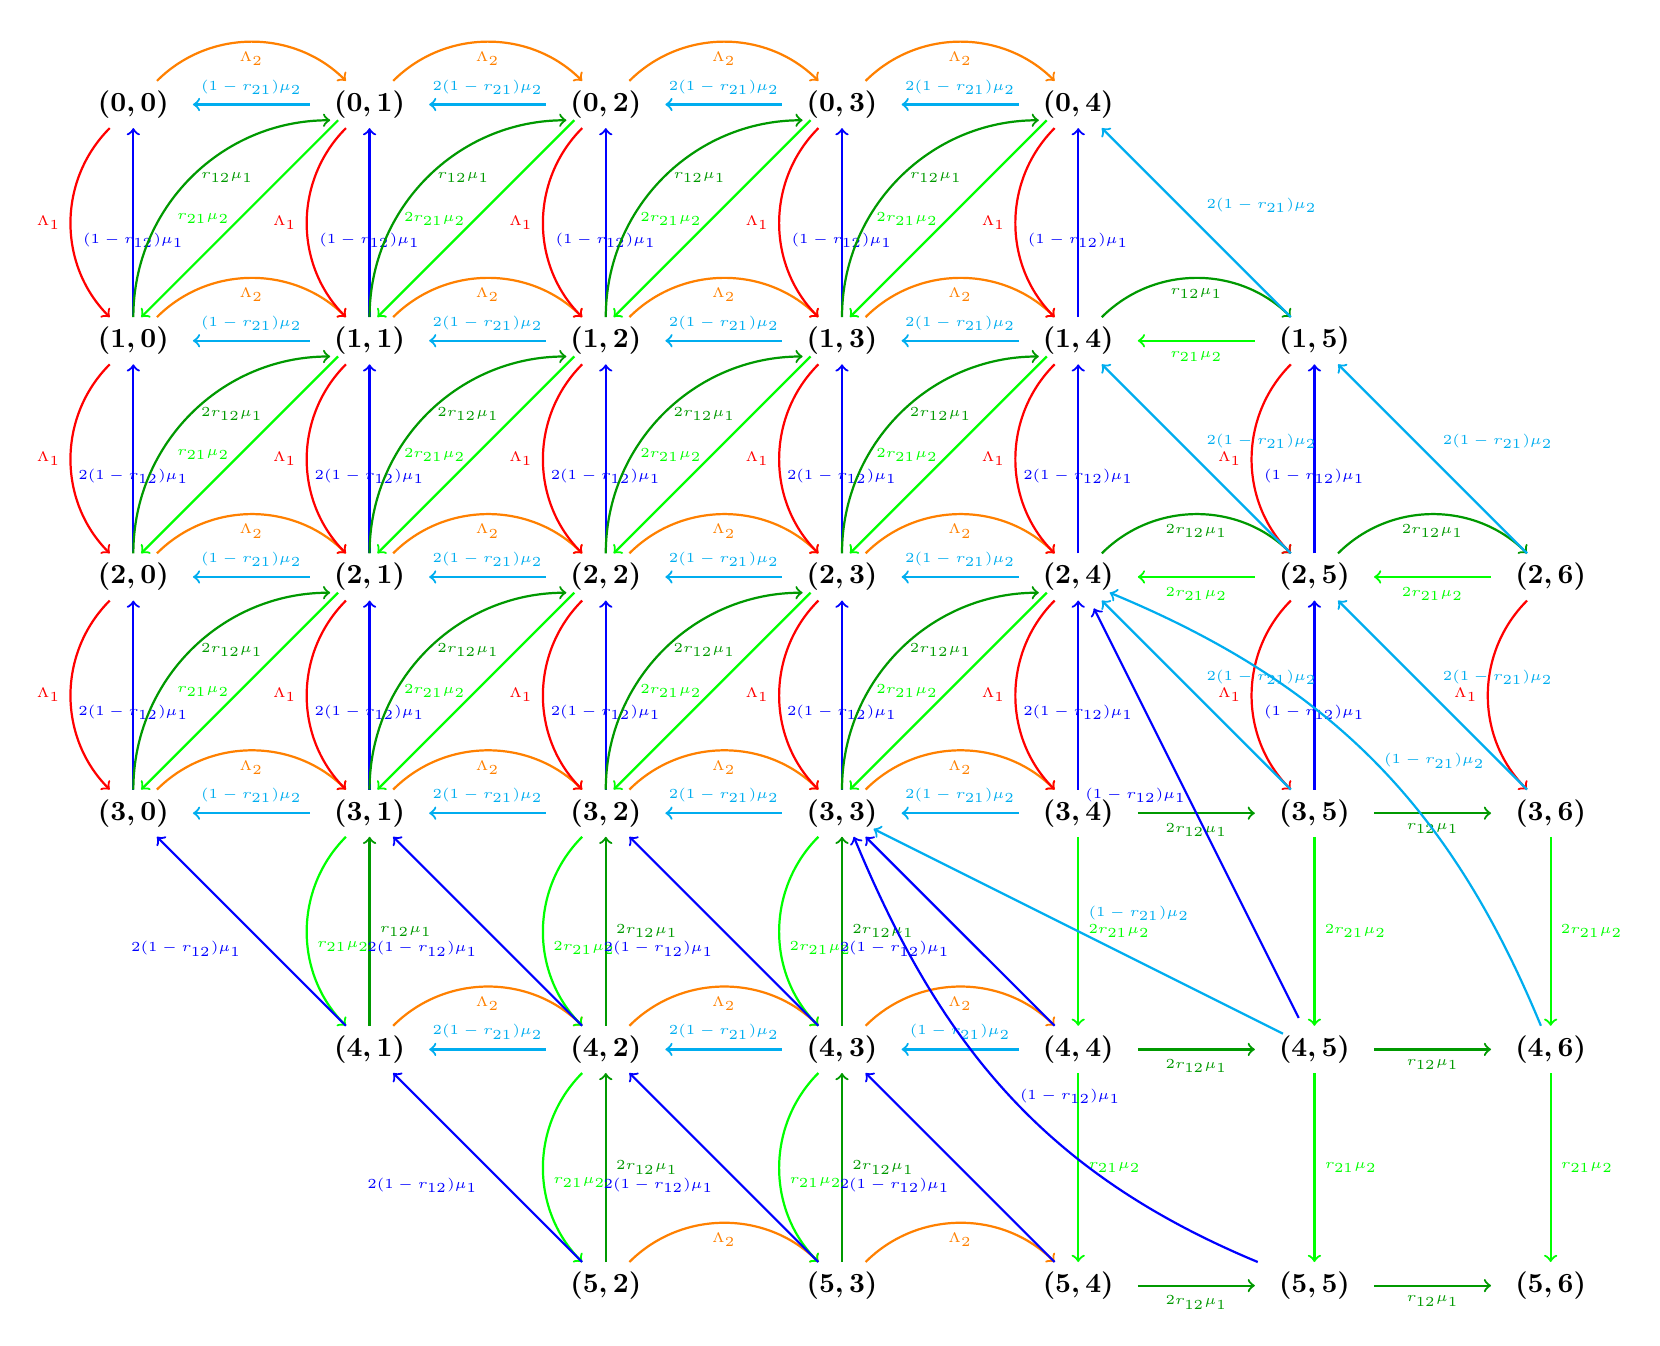
\begin{tikzpicture}
    \tikzstyle{state}=[minimum width=1.5cm, font=\boldmath];
    % First row
    \node (00) at (0,0) [state] {$(0, 0)$};
    \node (01) at ($(00)+(3,0)$) [state] {$(0, 1)$};
    \node (02) at ($(01)+(3,0)$) [state] {$(0, 2)$};
    \node (03) at ($(02)+(3,0)$) [state] {$(0, 3)$};
    \node (04) at ($(03)+(3,0)$) [state] {$(0, 4)$};

    % Second row
    \node (10) at ($(00)+(0,-3)$) [state] {$(1, 0)$};
    \node (11) at ($(10)+(3,0)$) [state] {$(1, 1)$};
    \node (12) at ($(11)+(3,0)$) [state] {$(1, 2)$};
    \node (13) at ($(12)+(3,0)$) [state] {$(1, 3)$};
    \node (14) at ($(13)+(3,0)$) [state] {$(1, 4)$};
    \node (15) at ($(14)+(3,0)$) [state] {$(1, 5)$};

    % Third row
    \node (20) at ($(10)+(0,-3)$) [state] {$(2, 0)$};
    \node (21) at ($(20)+(3,0)$) [state] {$(2, 1)$};
    \node (22) at ($(21)+(3,0)$) [state] {$(2, 2)$};
    \node (23) at ($(22)+(3,0)$) [state] {$(2, 3)$};
    \node (24) at ($(23)+(3,0)$) [state] {$(2, 4)$};
    \node (25) at ($(24)+(3,0)$) [state] {$(2, 5)$};
    \node (26) at ($(25)+(3,0)$) [state] {$(2, 6)$};

    % Fourth row
    \node (30) at ($(20)+(0,-3)$) [state] {$(3, 0)$};
    \node (31) at ($(30)+(3,0)$) [state] {$(3, 1)$};
    \node (32) at ($(31)+(3,0)$) [state] {$(3, 2)$};
    \node (33) at ($(32)+(3,0)$) [state] {$(3, 3)$};
    \node (34) at ($(33)+(3,0)$) [state] {$(3, 4)$};
    \node (35) at ($(34)+(3,0)$) [state] {$(3, 5)$};
    \node (36) at ($(35)+(3,0)$) [state] {$(3, 6)$};

    % Third row
    \node (41) at ($(31)+(0,-3)$) [state] {$(4, 1)$};
    \node (42) at ($(41)+(3,0)$) [state] {$(4, 2)$};
    \node (43) at ($(42)+(3,0)$) [state] {$(4, 3)$};
    \node (44) at ($(43)+(3,0)$) [state] {$(4, 4)$};
    \node (45) at ($(44)+(3,0)$) [state] {$(4, 5)$};
    \node (46) at ($(45)+(3,0)$) [state] {$(4, 6)$};

    % Third row
    \node (52) at ($(42)+(0,-3)$) [state] {$(5, 2)$};
    \node (53) at ($(52)+(3,0)$) [state] {$(5, 3)$};
    \node (54) at ($(53)+(3,0)$) [state] {$(5, 4)$};
    \node (55) at ($(54)+(3,0)$) [state] {$(5, 5)$};
    \node (56) at ($(55)+(3,0)$) [state] {$(5, 6)$};


    %%% TRANSITIONS

    % Right curve up
    \draw[draw=orange] (00) edge[out=45,in=135,->,thick] node [below, text=orange] {\tiny$\Lambda_2$} (01);
    \draw[draw=orange] (01) edge[out=45,in=135,->,thick] node [below, text=orange] {\tiny$\Lambda_2$} (02);
    \draw[draw=orange] (02) edge[out=45,in=135,->,thick] node [below, text=orange] {\tiny$\Lambda_2$} (03);
    \draw[draw=orange] (03) edge[out=45,in=135,->,thick] node [below, text=orange] {\tiny$\Lambda_2$} (04);

    \draw[draw=orange] (10) edge[out=45,in=135,->,thick] node [below, text=orange] {\tiny$\Lambda_2$} (11);
    \draw[draw=orange] (11) edge[out=45,in=135,->,thick] node [below, text=orange] {\tiny$\Lambda_2$} (12);
    \draw[draw=orange] (12) edge[out=45,in=135,->,thick] node [below, text=orange] {\tiny$\Lambda_2$} (13);
    \draw[draw=orange] (13) edge[out=45,in=135,->,thick] node [below, text=orange] {\tiny$\Lambda_2$} (14);
    \draw[draw=green!60!black] (14) edge[out=45,in=135,->,thick] node [below, text=green!60!black] {\tiny$r_{12}\mu_1$} (15);

    \draw[draw=orange] (20) edge[out=45,in=135,->,thick] node [below, text=orange] {\tiny$\Lambda_2$} (21);
    \draw[draw=orange] (21) edge[out=45,in=135,->,thick] node [below, text=orange] {\tiny$\Lambda_2$} (22);
    \draw[draw=orange] (22) edge[out=45,in=135,->,thick] node [below, text=orange] {\tiny$\Lambda_2$} (23);
    \draw[draw=orange] (23) edge[out=45,in=135,->,thick] node [below, text=orange] {\tiny$\Lambda_2$} (24);
    \draw[draw=green!60!black] (24) edge[out=45,in=135,->,thick] node [below, text=green!60!black] {\tiny$2r_{12}\mu_1$} (25);
    \draw[draw=green!60!black] (25) edge[out=45,in=135,->,thick] node [below, text=green!60!black] {\tiny$2r_{12}\mu_1$} (26);

    \draw[draw=orange] (30) edge[out=45,in=135,->,thick] node [below, text=orange] {\tiny$\Lambda_2$} (31);
    \draw[draw=orange] (31) edge[out=45,in=135,->,thick] node [below, text=orange] {\tiny$\Lambda_2$} (32);
    \draw[draw=orange] (32) edge[out=45,in=135,->,thick] node [below, text=orange] {\tiny$\Lambda_2$} (33);
    \draw[draw=orange] (33) edge[out=45,in=135,->,thick] node [below, text=orange] {\tiny$\Lambda_2$} (34);

    \draw[draw=orange] (41) edge[out=45,in=135,->,thick] node [below, text=orange] {\tiny$\Lambda_2$} (42);
    \draw[draw=orange] (42) edge[out=45,in=135,->,thick] node [below, text=orange] {\tiny$\Lambda_2$} (43);
    \draw[draw=orange] (43) edge[out=45,in=135,->,thick] node [below, text=orange] {\tiny$\Lambda_2$} (44);

    \draw[draw=orange] (52) edge[out=45,in=135,->,thick] node [below, text=orange] {\tiny$\Lambda_2$} (53);
    \draw[draw=orange] (53) edge[out=45,in=135,->,thick] node [below, text=orange] {\tiny$\Lambda_2$} (54);

    % Left
    \draw[draw=cyan] (00) edge[<-,thick] node [above, text=cyan] {\tiny$(1-r_{21})\mu_2$} (01);
    \draw[draw=cyan] (01) edge[<-,thick] node [above, text=cyan] {\tiny$2(1-r_{21})\mu_2$} (02);
    \draw[draw=cyan] (02) edge[<-,thick] node [above, text=cyan] {\tiny$2(1-r_{21})\mu_2$} (03);
    \draw[draw=cyan] (03) edge[<-,thick] node [above, text=cyan] {\tiny$2(1-r_{21})\mu_2$} (04);

    \draw[draw=cyan] (10) edge[<-,thick] node [above, text=cyan] {\tiny$(1-r_{21})\mu_2$} (11);
    \draw[draw=cyan] (11) edge[<-,thick] node [above, text=cyan] {\tiny$2(1-r_{21})\mu_2$} (12);
    \draw[draw=cyan] (12) edge[<-,thick] node [above, text=cyan] {\tiny$2(1-r_{21})\mu_2$} (13);
    \draw[draw=cyan] (13) edge[<-,thick] node [above, text=cyan] {\tiny$2(1-r_{21})\mu_2$} (14);
    \draw[draw=green] (14) edge[<-,thick] node [below, text=green] {\tiny$r_{21}\mu_2$} (15);

    \draw[draw=cyan] (20) edge[<-,thick] node [above, text=cyan] {\tiny$(1-r_{21})\mu_2$} (21);
    \draw[draw=cyan] (21) edge[<-,thick] node [above, text=cyan] {\tiny$2(1-r_{21})\mu_2$} (22);
    \draw[draw=cyan] (22) edge[<-,thick] node [above, text=cyan] {\tiny$2(1-r_{21})\mu_2$} (23);
    \draw[draw=cyan] (23) edge[<-,thick] node [above, text=cyan] {\tiny$2(1-r_{21})\mu_2$} (24);
    \draw[draw=green] (24) edge[<-,thick] node [below, text=green] {\tiny$2r_{21}\mu_2$} (25);
    \draw[draw=green] (25) edge[<-,thick] node [below, text=green] {\tiny$2r_{21}\mu_2$} (26);

    \draw[draw=cyan] (30) edge[<-,thick] node [above, text=cyan] {\tiny$(1-r_{21})\mu_2$} (31);
    \draw[draw=cyan] (31) edge[<-,thick] node [above, text=cyan] {\tiny$2(1-r_{21})\mu_2$} (32);
    \draw[draw=cyan] (32) edge[<-,thick] node [above, text=cyan] {\tiny$2(1-r_{21})\mu_2$} (33);
    \draw[draw=cyan] (33) edge[<-,thick] node [above, text=cyan] {\tiny$2(1-r_{21})\mu_2$} (34);

    \draw[draw=cyan] (41) edge[<-,thick] node [above, text=cyan] {\tiny$2(1-r_{21})\mu_2$} (42);
    \draw[draw=cyan] (42) edge[<-,thick] node [above, text=cyan] {\tiny$2(1-r_{21})\mu_2$} (43);
    \draw[draw=cyan] (43) edge[<-,thick] node [above, text=cyan] {\tiny$(1-r_{21})\mu_2$} (44);

    % Down curve left
    \draw[draw=red] (00) edge[out=-135,in=135,->,thick] node [left, text=red] {\tiny$\Lambda_1$} (10);
    \draw[draw=red] (10) edge[out=-135,in=135,->,thick] node [left, text=red] {\tiny$\Lambda_1$} (20);
    \draw[draw=red] (20) edge[out=-135,in=135,->,thick] node [left, text=red] {\tiny$\Lambda_1$} (30);

    \draw[draw=red] (01) edge[out=-135,in=135,->,thick] node [left, text=red] {\tiny$\Lambda_1$} (11);
    \draw[draw=red] (11) edge[out=-135,in=135,->,thick] node [left, text=red] {\tiny$\Lambda_1$} (21);
    \draw[draw=red] (21) edge[out=-135,in=135,->,thick] node [left, text=red] {\tiny$\Lambda_1$} (31);
    \draw[draw=green] (31) edge[out=-135,in=135,->,thick] node [below right, text=green] {\tiny$r_{21}\mu_2$} (41);

    \draw[draw=red] (02) edge[out=-135,in=135,->,thick] node [left, text=red] {\tiny$\Lambda_1$} (12);
    \draw[draw=red] (12) edge[out=-135,in=135,->,thick] node [left, text=red] {\tiny$\Lambda_1$} (22);
    \draw[draw=red] (22) edge[out=-135,in=135,->,thick] node [left, text=red] {\tiny$\Lambda_1$} (32);
    \draw[draw=green] (32) edge[out=-135,in=135,->,thick] node [below right, text=green] {\tiny$2r_{21}\mu_2$} (42);
    \draw[draw=green] (42) edge[out=-135,in=135,->,thick] node [below right, text=green] {\tiny$r_{21}\mu_2$} (52);

    \draw[draw=red] (03) edge[out=-135,in=135,->,thick] node [left, text=red] {\tiny$\Lambda_1$} (13);
    \draw[draw=red] (13) edge[out=-135,in=135,->,thick] node [left, text=red] {\tiny$\Lambda_1$} (23);
    \draw[draw=red] (23) edge[out=-135,in=135,->,thick] node [left, text=red] {\tiny$\Lambda_1$} (33);
    \draw[draw=green] (33) edge[out=-135,in=135,->,thick] node [below right, text=green] {\tiny$2r_{21}\mu_2$} (43);
    \draw[draw=green] (43) edge[out=-135,in=135,->,thick] node [below right, text=green] {\tiny$r_{21}\mu_2$} (53);

    \draw[draw=red] (04) edge[out=-135,in=135,->,thick] node [left, text=red] {\tiny$\Lambda_1$} (14);
    \draw[draw=red] (14) edge[out=-135,in=135,->,thick] node [left, text=red] {\tiny$\Lambda_1$} (24);
    \draw[draw=red] (24) edge[out=-135,in=135,->,thick] node [left, text=red] {\tiny$\Lambda_1$} (34);

    \draw[draw=red] (15) edge[out=-135,in=135,->,thick] node [left, text=red] {\tiny$\Lambda_1$} (25);
    \draw[draw=red] (25) edge[out=-135,in=135,->,thick] node [left, text=red] {\tiny$\Lambda_1$} (35);

    \draw[draw=red] (26) edge[out=-135,in=135,->,thick] node [left, text=red] {\tiny$\Lambda_1$} (36);

    % Right
    \draw[draw=green!60!black] (34) edge[->,thick] node [below, text=green!60!black] {\tiny$2r_{12}\mu_1$} (35);
    \draw[draw=green!60!black] (35) edge[->,thick] node [below, text=green!60!black] {\tiny$r_{12}\mu_1$} (36);

    \draw[draw=green!60!black] (44) edge[->,thick] node [below, text=green!60!black] {\tiny$2r_{12}\mu_1$} (45);
    \draw[draw=green!60!black] (45) edge[->,thick] node [below, text=green!60!black] {\tiny$r_{12}\mu_1$} (46);

    \draw[draw=green!60!black] (54) edge[->,thick] node [below, text=green!60!black] {\tiny$2r_{12}\mu_1$} (55);
    \draw[draw=green!60!black] (55) edge[->,thick] node [below, text=green!60!black] {\tiny$r_{12}\mu_1$} (56);

    % Down

    \draw[draw=green] (34) edge[->,thick] node [right, text=green] {\tiny$2r_{21}\mu_2$} (44);
    \draw[draw=green] (44) edge[->,thick] node [right, text=green] {\tiny$r_{21}\mu_2$} (54);

    \draw[draw=green] (35) edge[->,thick] node [right, text=green] {\tiny$2r_{21}\mu_2$} (45);
    \draw[draw=green] (45) edge[->,thick] node [right, text=green] {\tiny$r_{21}\mu_2$} (55);

    \draw[draw=green] (36) edge[->,thick] node [right, text=green] {\tiny$2r_{21}\mu_2$} (46);
    \draw[draw=green] (46) edge[->,thick] node [right, text=green] {\tiny$r_{21}\mu_2$} (56);

    % Up

    \draw[draw=blue] (10) edge[->,thick] node [below, text=blue] {\tiny$(1-r_{12})\mu_1$} (00);
    \draw[draw=blue] (20) edge[->,thick] node [below, text=blue] {\tiny$2(1-r_{12})\mu_1$} (10);
    \draw[draw=blue] (30) edge[->,thick] node [below, text=blue] {\tiny$2(1-r_{12})\mu_1$} (20);

    \draw[draw=blue] (11) edge[->,thick] node [below, text=blue] {\tiny$(1-r_{12})\mu_1$} (01);
    \draw[draw=blue] (21) edge[->,thick] node [below, text=blue] {\tiny$2(1-r_{12})\mu_1$} (11);
    \draw[draw=blue] (31) edge[->,thick] node [below, text=blue] {\tiny$2(1-r_{12})\mu_1$} (21);
    \draw[draw=green!60!black] (41) edge[->,thick] node [right, text=green!60!black] {\tiny$r_{12}\mu_1$} (31);

    \draw[draw=blue] (12) edge[->,thick] node [below, text=blue] {\tiny$(1-r_{12})\mu_1$} (02);
    \draw[draw=blue] (22) edge[->,thick] node [below, text=blue] {\tiny$2(1-r_{12})\mu_1$} (12);
    \draw[draw=blue] (32) edge[->,thick] node [below, text=blue] {\tiny$2(1-r_{12})\mu_1$} (22);
    \draw[draw=green!60!black] (42) edge[->,thick] node [right, text=green!60!black] {\tiny$2r_{12}\mu_1$} (32);
    \draw[draw=green!60!black] (52) edge[->,thick] node [right, text=green!60!black] {\tiny$2r_{12}\mu_1$} (42);

    \draw[draw=blue] (13) edge[->,thick] node [below, text=blue] {\tiny$(1-r_{12})\mu_1$} (03);
    \draw[draw=blue] (23) edge[->,thick] node [below, text=blue] {\tiny$2(1-r_{12})\mu_1$} (13);
    \draw[draw=blue] (33) edge[->,thick] node [below, text=blue] {\tiny$2(1-r_{12})\mu_1$} (23);
    \draw[draw=green!60!black] (43) edge[->,thick] node [right, text=green!60!black] {\tiny$2r_{12}\mu_1$} (33);
    \draw[draw=green!60!black] (53) edge[->,thick] node [right, text=green!60!black] {\tiny$2r_{12}\mu_1$} (43);

    \draw[draw=blue] (14) edge[->,thick] node [below, text=blue] {\tiny$(1-r_{12})\mu_1$} (04);
    \draw[draw=blue] (24) edge[->,thick] node [below, text=blue] {\tiny$2(1-r_{12})\mu_1$} (14);
    \draw[draw=blue] (34) edge[->,thick] node [below, text=blue] {\tiny$2(1-r_{12})\mu_1$} (24);

    \draw[draw=blue] (25) edge[->,thick] node [below, text=blue] {\tiny$(1-r_{12})\mu_1$} (15);
    \draw[draw=blue] (35) edge[->,thick] node [below, text=blue] {\tiny$(1-r_{12})\mu_1$} (25);


    % Diagonal backslash
    \draw[draw=cyan] (15) edge[->,thick] node [above right, text=cyan] {\tiny$2(1-r_{21})\mu_2$} (04);

    \draw[draw=cyan] (25) edge[->,thick] node [above right, text=cyan] {\tiny$2(1-r_{21})\mu_2$} (14);
    \draw[draw=cyan] (26) edge[->,thick] node [above right, text=cyan] {\tiny$2(1-r_{21})\mu_2$} (15);

    \draw[draw=cyan] (35) edge[->,thick] node [above right, text=cyan] {\tiny$2(1-r_{21})\mu_2$} (24);
    \draw[draw=cyan] (36) edge[->,thick] node [above right, text=cyan] {\tiny$2(1-r_{21})\mu_2$} (25);

    \draw[draw=blue] (41) edge[->,thick] node [below left, text=blue] {\tiny$2(1-r_{12})\mu_1$} (30);
    \draw[draw=blue] (42) edge[->,thick] node [below left, text=blue] {\tiny$2(1-r_{12})\mu_1$} (31);
    \draw[draw=blue] (43) edge[->,thick] node [below left, text=blue] {\tiny$2(1-r_{12})\mu_1$} (32);
    \draw[draw=blue] (44) edge[->,thick] node [below left, text=blue] {\tiny$2(1-r_{12})\mu_1$} (33);

    \draw[draw=blue] (52) edge[->,thick] node [below left, text=blue] {\tiny$2(1-r_{12})\mu_1$} (41);
    \draw[draw=blue] (53) edge[->,thick] node [below left, text=blue] {\tiny$2(1-r_{12})\mu_1$} (42);
    \draw[draw=blue] (54) edge[->,thick] node [below left, text=blue] {\tiny$2(1-r_{12})\mu_1$} (43);

    % Diagonal forwardslash curve
    \draw[draw=green!60!black] (10) edge[out=90,in=180,->,thick] node [right, text=green!60!black] {\tiny$r_{12}\mu_1$} ($(01)+(-0.5,-0.2)$);
    \draw[draw=green!60!black] (11) edge[out=90,in=180,->,thick] node [right, text=green!60!black] {\tiny$r_{12}\mu_1$} ($(02)+(-0.5,-0.2)$);
    \draw[draw=green!60!black] (12) edge[out=90,in=180,->,thick] node [right, text=green!60!black] {\tiny$r_{12}\mu_1$} ($(03)+(-0.5,-0.2)$);
    \draw[draw=green!60!black] (13) edge[out=90,in=180,->,thick] node [right, text=green!60!black] {\tiny$r_{12}\mu_1$} ($(04)+(-0.5,-0.2)$);

    \draw[draw=green!60!black] (20) edge[out=90,in=180,->,thick] node [right, text=green!60!black] {\tiny$2r_{12}\mu_1$} ($(11)+(-0.5,-0.2)$);
    \draw[draw=green!60!black] (21) edge[out=90,in=180,->,thick] node [right, text=green!60!black] {\tiny$2r_{12}\mu_1$} ($(12)+(-0.5,-0.2)$);
    \draw[draw=green!60!black] (22) edge[out=90,in=180,->,thick] node [right, text=green!60!black] {\tiny$2r_{12}\mu_1$} ($(13)+(-0.5,-0.2)$);
    \draw[draw=green!60!black] (23) edge[out=90,in=180,->,thick] node [right, text=green!60!black] {\tiny$2r_{12}\mu_1$} ($(14)+(-0.5,-0.2)$);

    \draw[draw=green!60!black] (30) edge[out=90,in=180,->,thick] node [right, text=green!60!black] {\tiny$2r_{12}\mu_1$} ($(21)+(-0.5,-0.2)$);
    \draw[draw=green!60!black] (31) edge[out=90,in=180,->,thick] node [right, text=green!60!black] {\tiny$2r_{12}\mu_1$} ($(22)+(-0.5,-0.2)$);
    \draw[draw=green!60!black] (32) edge[out=90,in=180,->,thick] node [right, text=green!60!black] {\tiny$2r_{12}\mu_1$} ($(23)+(-0.5,-0.2)$);
    \draw[draw=green!60!black] (33) edge[out=90,in=180,->,thick] node [right, text=green!60!black] {\tiny$2r_{12}\mu_1$} ($(24)+(-0.5,-0.2)$);

    % Diagonal forwardslash
    \draw[draw=green] ($(01)+(-0.4,-0.2)$) edge[->,thick] node [left, text=green] {\tiny$r_{21}\mu_2$} ($(10)+(0.1,0.3)$);
    \draw[draw=green] ($(02)+(-0.4,-0.2)$) edge[->,thick] node [left, text=green] {\tiny$2r_{21}\mu_2$} ($(11)+(0.1,0.3)$);
    \draw[draw=green] ($(03)+(-0.4,-0.2)$) edge[->,thick] node [left, text=green] {\tiny$2r_{21}\mu_2$} ($(12)+(0.1,0.3)$);
    \draw[draw=green] ($(04)+(-0.4,-0.2)$) edge[->,thick] node [left, text=green] {\tiny$2r_{21}\mu_2$} ($(13)+(0.1,0.3)$);

    \draw[draw=green] ($(11)+(-0.4,-0.2)$) edge[->,thick] node [left, text=green] {\tiny$r_{21}\mu_2$} ($(20)+(0.1,0.3)$);
    \draw[draw=green] ($(12)+(-0.4,-0.2)$) edge[->,thick] node [left, text=green] {\tiny$2r_{21}\mu_2$} ($(21)+(0.1,0.3)$);
    \draw[draw=green] ($(13)+(-0.4,-0.2)$) edge[->,thick] node [left, text=green] {\tiny$2r_{21}\mu_2$} ($(22)+(0.1,0.3)$);
    \draw[draw=green] ($(14)+(-0.4,-0.2)$) edge[->,thick] node [left, text=green] {\tiny$2r_{21}\mu_2$} ($(23)+(0.1,0.3)$);

    \draw[draw=green] ($(21)+(-0.4,-0.2)$) edge[->,thick] node [left, text=green] {\tiny$r_{21}\mu_2$} ($(30)+(0.1,0.3)$);
    \draw[draw=green] ($(22)+(-0.4,-0.2)$) edge[->,thick] node [left, text=green] {\tiny$2r_{21}\mu_2$} ($(31)+(0.1,0.3)$);
    \draw[draw=green] ($(23)+(-0.4,-0.2)$) edge[->,thick] node [left, text=green] {\tiny$2r_{21}\mu_2$} ($(32)+(0.1,0.3)$);
    \draw[draw=green] ($(24)+(-0.4,-0.2)$) edge[->,thick] node [left, text=green] {\tiny$2r_{21}\mu_2$} ($(33)+(0.1,0.3)$);

    % Extra transitions
    \draw[draw=blue] ($(45)+(-0.2,0.4)$) edge[->,thick] node [above left,text=blue] {\tiny$(1-r_{12})\mu_1$} ($(24)+(0.2,-0.4)$);
    \draw[draw=cyan] ($(45)+(-0.4,0.2)$) edge[->,thick] node [above right,text=cyan] {\tiny$(1-r_{21})\mu_2$} ($(33)+(0.4,-0.2)$);
    \draw[draw=cyan] (46) edge[out=112.5,in=-22.5,->,thick] node [right,text=cyan] {\tiny$(1-r_{21})\mu_2$} ($(24)+(0.4,-0.2)$);
    \draw[draw=blue] (55) edge[out=157.5,in=-67.5,->,thick] node [right,text=blue] {\tiny$(1-r_{12})\mu_1$} ($(33)+(0.15,-0.3)$);

\end{tikzpicture}

\end{document}
